\lysh{14654}{4}

\begin{alist}
\item Το τριώνυμο $x^2 - 3x + 2$ έχει $\alpha = 1$, $\beta = -3$, $\gamma = 2$ και διακρίνουσα: $\Delta = \beta^2 - 4\alpha\gamma = 1 > 0$.
Οι ρίζες του τριωνύμου είναι οι:
\[x_{1,2} = \dfrac{-\beta \pm \sqrt{\Delta}}{2\alpha} = \dfrac{3 \pm 1}{2} \Leftrightarrow x_1 = 1 \text{ και } x_2 = 2.\]
Το πρόσημο του τριωνύμου φαίνεται στον παρακάτω πίνακα.

\begin{center}
\begin{tikzpicture}
\tikzset{t style/.style = {style = dashed}}
\tkzTabInit[color,lgt=3,espcl=2,colorC = maincolor!40,
colorL = maincolor!20,
colorV = maincolor!40]%
{$x$ / .8,$x^2 - 3x + 2$ /0.8}%
{$-\infty$,$1$,$2$,$+\infty$}%
\tkzTabLine{ , $+$, z
, $-$ , z
, $+$ , }
\end{tikzpicture}
\end{center}

Από τον πίνακα προσήμων συμπεραίνουμε ότι το τριώνυμο είναι θετικό για
$x \in (-\infty, 1) \cup (2, +\infty)$ και αρνητικό για $x \in (1, 2)$.

\item 
\begin{rlist}
\item Δεδομένου ότι $(\alpha^2 - 3\alpha + 2)(\beta^2 - 3\beta + 2) < 0$, διακρίνουμε δυο περιπτώσεις:

1η περίπτωση: $\alpha^2 - 3\alpha + 2 < 0$ και $\beta^2 - 3\beta + 2 > 0$,
Από το $\alpha)$ ερώτημα $\alpha \in (1, 2)$ και $\beta \in (-\infty, 1) \cup (2, +\infty)$, δηλαδή $\alpha > 1$ και αφού $\alpha < \beta$
και είναι $\beta > 2$, συνεπώς $\alpha - 1$ και $\beta - 2$ είναι θετικοί, άρα ομόσημοι.

2η περίπτωση: $\alpha^2 - 3\alpha + 2 > 0$ και $\beta^2 - 3\beta + 2 < 0$,
Από το $\alpha)$ ερώτημα $\alpha \in (-\infty, 1) \cup (2, +\infty)$ και $\beta \in (1, 2)$ δηλαδή $\beta < 2$ και αφού $\alpha < \beta$
θα είναι $\alpha < 1$, συνεπώς $\alpha - 1$ και $\beta - 2$ είναι αρνητικοί άρα ομόσημοι.

\item Αφού $\alpha - 1$ και $\beta - 2$ είναι ομόσημοι, έχουμε ότι $(\alpha - 1)(\beta - 2) > 0$, οπότε:
\[|(\alpha - 1)(\beta - 2)| = (\alpha - 1)(\beta - 2).\]
\end{rlist}
\end{alist}
